
%!TEX root = ../thesis.tex
%*******************************************************************************
%****************************** Second Chapter *********************************
%*******************************************************************************

\chapter{Concept}

\ifpdf
    \graphicspath{{Chapter2/Figs/Raster/}{Chapter2/Figs/PDF/}{Chapter2/Figs/}}
\else
    \graphicspath{{Chapter2/Figs/Vector/}{Chapter2/Figs/}}
\fi

\fbox{
    \parbox{\textwidth}
    {
        Architecture guidelines for stable Deep Convolutional GANs
        \begin{itemize}
            \item Replace any pooling layers with strided convolutions (discriminator) and fractional-strided convolutions (generator).
            \item Use batchnorm in both the generator and the discriminator.
            \item Remove fully connected hidden layers for deeper architectures.
            \item Use ReLU activation in generator for all layers except for the output, which uses Tanh.
            \item Use LeakyReLU activation in the discriminator for all layers.
        \end{itemize}
    }
}

\pagebreak

\section{Bayesian convolutional neural networks with variational inference}
In this section, we explain our algorithm of building a \ac{cnn} with probability distributions over its weights in each filter, as seen in Figure \ref{fig:filter_scalar}, and apply variational inference, i.e. \textit{Bayes by Backprop}, to compute the intractable true posterior probability distribution, as described in the previous section. Notably, a fully Bayesian perspective on a \ac{cnn} is for most \ac{cnn} architectures not accomplished by merely placing probability distributions over weights in convolutional layers; it also requires probability distributions over weights in fully-connected layers (see Figure \ref{fig:CNNwithdist_grey}). 
%
\begin{figure}[H] 
\centering
\begin{minipage}{.4\textwidth}
\centering
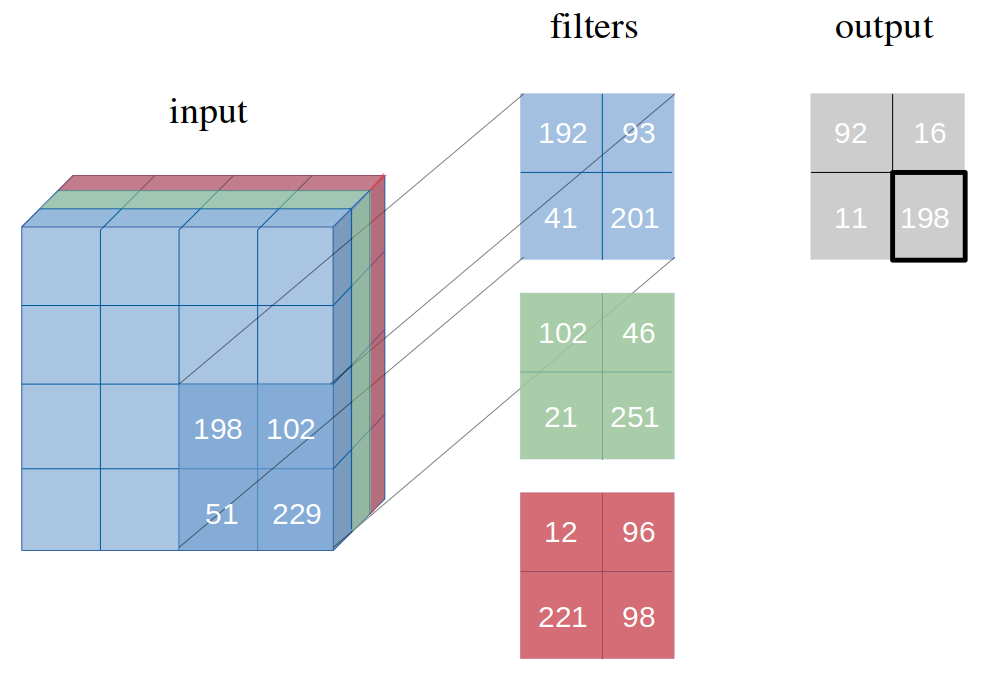
\includegraphics[width=\linewidth]{Chapter4/Figs/filter_scalars.png}
\end{minipage}
%
\begin{minipage}{.4\textwidth}
\centering
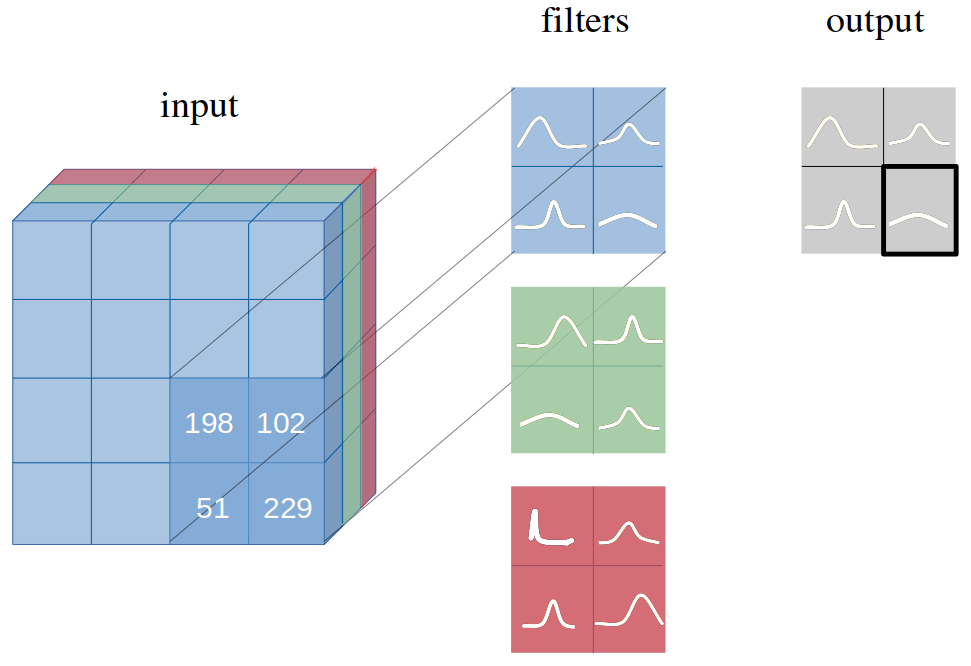
\includegraphics[width=\linewidth]{Chapter4/Figs/CNNwithdist.png}
\end{minipage}
\caption{Input image with exemplary pixel values, filters, and corresponding output with point-estimates (top) and probability distributions (bottom) over weights.}
\label{fig:filter_scalar}
\end{figure} 
%
\begin{figure}[b!] 
\begin{center}
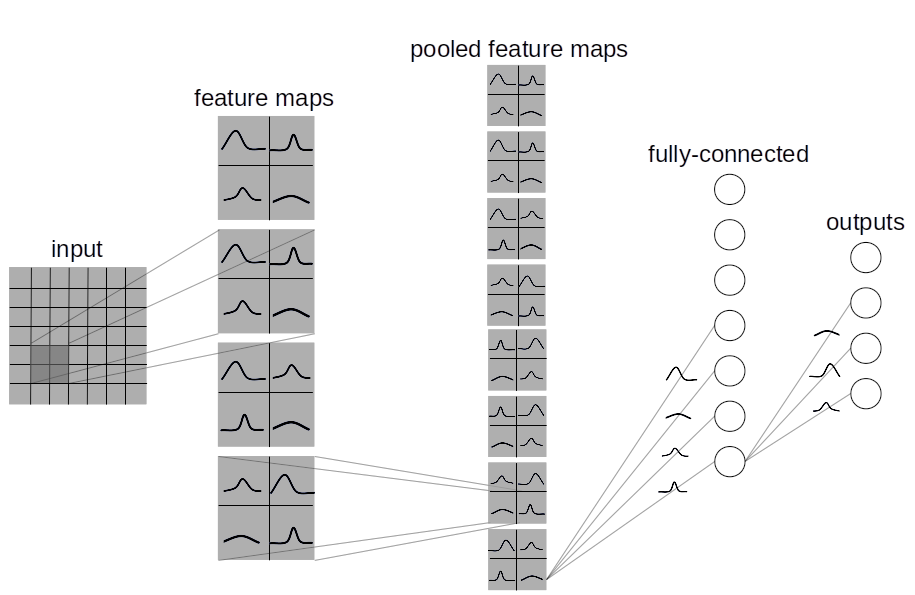
\includegraphics[width=\linewidth]{Chapter4/Figs/CNNwithdist_grey.png}}
\caption{Fully Bayesian perspective of an exemplary \ac{cnn}. Weights in filters of convolutional layers, and weights in fully-connected layers have the form of a probability distribution.}
\label{fig:CNNwithdist_grey}
\end{center}
\end{figure} 
%
\subsection{Local reparameterization trick for convolutional layers}
We utilise the local reparameterization trick \cite{kingma2015variational} and apply it to \acp{cnn}. Following \cite{kingma2015variational,neklyudov2018variance}, we do not sample the weights $w$, but we sample instead layer activations $b$ due to its consequent computational acceleration. The variational posterior probability distribution $q_{\theta}(w_{ijhw}|\mathcal{D})=\mathcal{N}(\mu_{ijhw},\alpha_{ijhw}\mu^2_{ijhw})$ (where $i$ and $j$ are the input, respectively output layers, $h$ and $w$ the height, respectively width of any given filter) allows to implement the local reparamerization trick in convolutional layers. This results in the subsequent equation for convolutional layer activations $b$:
\begin{equation}
    b_j=A_i\ast \mu_i+\epsilon_j\odot \sqrt{A^2_i\ast (\alpha_i\odot \mu^2_i)}
\end{equation}
where $\epsilon_j \sim \mathcal{N}(0,1)$, $A_i$ is the receptive field, $\ast$ signalises the convolutional operation, and $\odot$ the component-wise multiplication.

\subsection{Applying two sequential convolutional operations (mean and variance)}
The crux of equipping a \ac{cnn} with probability distributions over weights instead of single point-estimates and being able to update the variational posterior probability distribution $q_{\theta}(w|\mathcal{D})$ by backpropagation lies in applying \textit{two} convolutional operations whereas filters with single point-estimates apply \textit{one}. As explained in the previous section, we deploy the local reparametrization trick and sample from the output $b$. Since the output $b$ is a function of mean $\mu_{ijwh}$ and variance $\alpha_{ijhw}\mu^2_{ijhw}$ among others, we are then able to compute the two variables determining a Gaussian probability distribution, namely mean $\mu_{ijhw}$ and variance $\alpha_{ijhw}\mu^2_{ijhw}$, separately. 
\newline We do this in two convolutional operations: in the first, we treat the output $b$ as an output of a \ac{cnn} updated by frequentist inference. We optimize with Adam \cite{kingma2014adam} towards a single point-estimate which makes the validation accuracy of classifications increasing. We interpret this single point-estimate as the mean $\mu_{ijwh}$ of the variational posterior probability distributions $q_{\theta}(w|\mathcal{D})$. In the second convolutional operation, we learn the variance $\alpha_{ijhw}\mu^2_{ijhw}$. As this formulation of the variance includes the mean $\mu_{ijwh}$, only $\alpha_{ijhw}$ needs to be learned in the second convolutional operation \cite{molchanov2017variational}. In this way, we ensure that only one parameter is updated per convolutional operation, exactly how it would have been with a \ac{cnn} updated by frequentist inference. 
\newline In other words, while we learn in the first convolutional operation the MAP of the variational posterior probability distribution $q_{\theta}(w|\mathcal{D})$, we observe in the second convolutional operation how much values for weights $w$ deviate from this MAP. This procedure is repeated in the fully-connected layers. In addition, to accelerate computation, to ensure a positive non-zero variance $\alpha_{ijhw}\mu^2_{ijhw}$, and to enhance accuracy, we learn $\log \alpha_{ijhw}$ and use the \textit{Softplus} activation function as further described in the Experiments section.
%
\section{Uncertainty estimation in \acp{cnn}}
In classification tasks, we are interested in the predictive distribution $p_{\mathcal{D}}(y^*|x^*)$, where $x^*$ is an unseen data example and $y^*$ its predicted class. For a Bayesian neural network, this quantity is given by:
\begin{align}
p_{ \mathcal{D}}(y^*|x^*) = \int p_{w}(y^*|x^*) \ p_{\mathcal{D}}(w) \ dw
\end{align}
%
In \textit{Bayes by Backprop}, Gaussian distributions $q_{\theta}(w|\mathcal{D}) \sim \mathcal{N}(w|\mu, \sigma^2)$, where $\theta = \{ \mu, \sigma \}$ are learned with some dataset $\mathcal{D} = \{ x_{i}, y_{i} \}_{i=1}^{n}$ as we explained previously. Due to the discrete and finite nature of most classification tasks, the predictive distribution is commonly assumed to be a categorical. Incorporating this aspect into the predictive distribution gives us
\begin{align}
p_{\mathcal{D}}(y^*|x^*)& = \int \text{Cat}(y^*|f_w(x^*)) \mathcal{N}(w|\mu, \sigma^2) \ dw\\
&=  \int \prod_{c=1}^{C} f(x_{c}^*|w)^{y_{c}^*} \frac{1}{\sqrt{2\pi \sigma^2}} e^{-\frac{(w - \mu)^2}{2\sigma^2}} \ dw 
\end{align}
where $C$ is the total number of classes and $\sum_c f(x_{c}^*|w) = 1$.
\newline As there is no closed-form solution due to the lack of conjugacy between categorical and Gaussian distributions, we cannot recover this distribution. However, we can construct an unbiased estimator of the expectation by sampling from $q_{\theta}(w|\mathcal{D})$:
\begin{align}
\mathbb{E}_{q}[p_{\mathcal{D}}(y^*|x^*)] &= \int q_{\theta}(w|\mathcal{D}) \ p_w(y|x) \ dw \\ & \approx \frac{1}{T}\sum_{t=1}^{T} p_{w_t}(y^*|x^*)
\end{align}
where $T$ is the pre-defined number of samples.
This estimator allows us to evaluate the uncertainty of our predictions by the definition of variance, hence called \textit{predictive variance} and denoted as $\text{Var}_q$:
\begin{align} \label{variance}
\text{Var}_q\big( p(y^*|x^*) \big) = \mathbb{E}_q[yy^T] - \mathbb{E}_q[y]\mathbb{E}_q[y]^T
\end{align}
This quantity can be decomposed into the aleatoric and epistemic uncertainty \cite{kendall2017uncertainties,kwon2018uncertainty}. 
\begin{equation}
    \begin{aligned}
    \text{Var}_q\big( p(y^*|x^*) \big) &= \underbrace{\frac{1}{T} \sum_{t=1}^T \text{diag}(\hat{p}_t)-\hat{p}_t \ \hat{p}_t^T}_\text{aleatoric} \\ &+ \underbrace{\frac{1}{T}\sum_{t=1}^T (\hat{p}_t - \Bar{p}) (\hat{p}_t - \Bar{p})^T}_\text{epistemic}
    \end{aligned}
\end{equation}
where $\Bar{p} = \frac{1}{T}\sum_{t=1}^T \hat{p}_t$ and $\hat{p}_t = \text{Softmax}\big ( f_{w_{t}}(x^*) \big )$.
\newline It is of paramount importance that uncertainty is split into aleatoric and epistemic quantities since it allows the modeler to evaluate the room for improvements: while aleatoric uncertainty (also known as statistical uncertainty) is merely a measure for the variation of ("noisy") data, epistemic uncertainty is caused by the model. Hence, a modeler can see whether the quality of the data is low (i.e. high aleatoric uncertainty), or the model itself is the cause for poor performances (i.e. high epistemic uncertainty). The former can be improved by gathering more data, whereas the latter requests to refine the model \cite{der2009aleatory}.
